% !TEX root = ../../main.tex
\section{Статистичний аналіз лінійної регресійної моделі}
\subsection{Властивості оцінок параметрів}
Будемо досліджувати властивості оцінок параметрів $\vec{\beta}$, отриманих за допомогою МНК
за формулою (\ref{regr_coef}): $\vec{\beta}^* = (F^T F)^{-1} F^T \vec{\eta}$.
\begin{proposition}\label{regr_unbiased}
    Вектор $\vec{\beta}^*$ має гауссівський розподіл та є незміщеною оцінкою $\vec{\beta}$.
\end{proposition}
\begin{proof}
    $\vec{\beta}^* - \vec{\beta} = (F^T F)^{-1} F^T \vec{\eta} - \vec{\beta} = 
    \left[\vec{\eta} = F\vec{\beta} + \vec{\varepsilon}\right] =
    (F^T F)^{-1} F^T (F\vec{\beta} + \vec{\varepsilon}) - \vec{\beta} = $\\
    $= (F^T F)^{-1} F^T F \vec{\beta} + (F^T F)^{-1} F^T \vec{\varepsilon} - \vec{\beta} = 
    \vec{\beta} + (F^T F)^{-1} F^T \vec{\varepsilon} - \vec{\beta} = (F^T F)^{-1} F^T \vec{\varepsilon}$.
    Оскільки, за припущенням, $\vec{\varepsilon} \sim \mathrm{N}(\vec{0}, \sigma^2 \mathbb{I})$,
    то $\vec{\beta}^* = (F^T F)^{-1} F^T \vec{\varepsilon} + \vec{\beta}$ також має гауссівський розподіл.
    Знайдемо параметри цього розподілу:
    \begin{gather*}
        \E\vec{\beta}^* = \E (F^T F)^{-1} F^T \vec{\varepsilon} + \vec{\beta} = 
        (F^T F)^{-1} F^T \E\vec{\varepsilon} + \vec{\beta} = \vec{\beta} \\
        \K\vec{\beta}^* = (F^T F)^{-1} F^T \K\vec{\varepsilon} \left((F^T F)^{-1} F^T\right)^T = 
        (F^T F)^{-1} F^T \cdot \sigma^2 \mathbb{I} \cdot F (F^T F)^{-1} = \sigma^2 (F^T F)^{-1}
    \end{gather*}
    Отже, $\vec{\beta}^* \sim \mathrm{N}(\vec{\beta}, \sigma^2 A^{-1})$, де $A = F^T F$.
    Це, зокрема, пояснює назву матриці $(F^T F)^{-1}$ --- <<дисперсійна>>.
    Зауважимо, що значення $\sigma^2$ невідоме. Пізніше буде досліджено його оцінку.
\end{proof}
\begin{proposition}[теорема Гаусса-Маркова] Незміщена оцінка $\vec{\beta}^*$, що знайдена за формулою
    (\ref{regr_coef}), є ефективною в класі незміщених лінійних оцінок.
\end{proposition}
\begin{proof}
    Нехай існує інша незміщена оцінка $\vec{\beta}^{**}$. Оскільки розглядається клас лінійних оцінок, то
    $\vec{\beta}^{**} = C\vec{\eta}$ для деякої матриці $C$. Розпишемо параметри розподілу цієї оцінки.
    $$\vec{\beta} = \E\vec{\beta}^{**} = \E ( C (F \vec{\beta} + \vec{\varepsilon})) = 
    C F \vec{\beta} + C\E\vec{\varepsilon} = C F \vec{\beta}$$ звідки $CF = \mathbb{I}$ --- одинична матриця.
    \begin{gather*}
        \K \vec{\beta}^{**} = \E(\vec{\beta}^{**} - \E\vec{\beta}^{**})(\vec{\beta}^{**} - \E\vec{\beta}^{**})^T = 
        \E (C\vec{\eta} - \vec{\beta})(C\vec{\eta} - \vec{\beta})^T = \\
        = \E (C\vec{\eta} - C F\vec{\beta})(C\vec{\eta} - C F\vec{\beta})^T = 
        C \E (\vec{\eta} - F\vec{\beta})(\vec{\eta} - F\vec{\beta})^T C^T = 
        C \E \vec{\varepsilon}\vec{\varepsilon}^T C^T = \sigma^2 C C^T
    \end{gather*}
    Нехай $D = C - A^{-1}F^T = C - (F^T F)^{-1} F^T$, тоді $C = A^{-1}F^T + D$.
    Маємо $\mathbb{I} = C F = A^{-1}F^T F + D F = (F^T F)^{-1} F^T F + D F = \mathbb{I} + DF$,
    звідки $D F = 0$. Підставимо цей вираз для $C$ в вираз для $\K \vec{\beta}^{**}$:
    \begin{gather*}
        \K \vec{\beta}^{**} = \sigma^2 C C^T = \sigma^2 (A^{-1}F^T + D)(A^{-1}F^T + D)^T = \\ =
        \sigma^2 \left(
            (A^{-1}F^T)(A^{-1}F^T)^T + D (A^{-1}F^T)^T + (A^{-1}F^T)D^T + D D^T
        \right) = \\ =
        \sigma^2 \left(
            A^{-1}F^T F (A^T)^{-1} + D F (A^T)^{-1} + A^{-1} (DF)^T + D D^T
        \right) = \\ =
        \sigma^2 \left(
            A^{-1} + D D^T
        \right) = \K \vec{\beta}^* + \sigma^2 D D^T
    \end{gather*}
    Звідси $\K \vec{\beta}^{**} - \K \vec{\beta}^* = \sigma^2 D D^T$. Оскільки
    $\forall \; \vec{x} : \left(D D^T \vec{x}, \vec{x}\right) = \left(D^T\vec{x}, D^T\vec{x}\right) = 
    \Vert D^T \vec{x} \Vert^2 \geq 0$, то матриця $\sigma^2 D D^T \geq 0$ (невід'ємно визначена).
    Отже, $\K \vec{\beta}^{**} - \K \vec{\beta}^* \geq 0$, що доводить ефективність $\vec{\beta}^*$.
\end{proof}
\begin{remark}
    Дослідження ефективності лише в класі незміщених лінійних оцінок інтуїтивно пояснюється тим, що якщо $\vec{\eta}$ лінійно залежить від $\vec{\beta}$,
    то й усі <<хороші>> оцінки $\vec{\beta}$ будуть лінійно залежати від $\vec{\eta}$.
\end{remark}
\begin{proposition}
    Незміщена оцінка $\vec{\beta}^*$, що знайдена за формулою
    (\ref{regr_coef}), є конзистентною.
\end{proposition}
\begin{proof}
    В твердженні \ref{regr_unbiased} було показано, що
    $\vec{\beta}^* = (F^T F)^{-1} F^T \vec{\varepsilon} + \vec{\beta}$ і $\vec{\beta}^* - \vec{\beta} \sim \mathrm{N}(\vec{0},\sigma^2 A^{-1})$.
    Матриця $A^{-1}$ залежить від $n$, тому застосувати закон великих чисел
    для випадкових векторів в тому формулюванні, яке було наведено (ст. \pageref{multivar_lln}), не вдасться.
    Натомість, буде достатньо довести, що для $i=1,..., m$ $\D\left(\beta^*_i - \beta_i\right) = \D\beta^*_i \to 0 , n \to \infty$. 
    
    Без втрати загальності
    можна вважати, що $\sigma = 1$, тоді на діагоналі матриці $A^{-1}$ будуть знаходитися дисперсії $\D\beta_i^*$.
    $\forall \; i = 1,..., m : \D\beta_i^* \leq \sum\limits_{k=1}^m \D\beta_k^* = \mathrm{tr} A^{-1}$.
    Нехай $\lambda_1 \geq ... \geq \lambda_m > 0$ --- власні числа матриці $A$, тоді
    $\mathrm{tr} A^{-1} = \frac{1}{\lambda_1} + ... + \frac{1}{\lambda_m} = 
    \frac{
        \frac{\lambda_1 \lambda_2 ... \lambda_m}{\lambda_1} + 
        \frac{\lambda_1 \lambda_2 ... \lambda_m}{\lambda_2} + ... +
        \frac{\lambda_1 \lambda_2 ... \lambda_m}{\lambda_m}
    }{\lambda_1 \lambda_2 ... \lambda_m}$. З лінійної алгебри відомо, що
    $\lambda_1 \lambda_2 ... \lambda_m = \det A$, а доданки $\frac{\lambda_1 \lambda_2 ... \lambda_m}{\lambda_j}$ в чисельнику --- визначники мінорів матриці $A$,
    що отримані викреслюванням $j$-того стовпця та рядка --- це випливає з формули для характеристичного полінома
    $\det(A - \lambda \mathbb{I})$ та фактів, що його коефіцієнти не залежать від базису, а в деякому базисі матриця $A$ є діагональною.
    Тепер можна оцінити $\frac{\lambda_1 \lambda_2 ... \lambda_m}{\lambda_1} + 
    \frac{\lambda_1 \lambda_2 ... \lambda_m}{\lambda_2} + ... +
    \frac{\lambda_1 \lambda_2 ... \lambda_m}{\lambda_m} \leq m \cdot \underset{j=1,...,m}{\max}\frac{\lambda_1 \lambda_2 ... \lambda_m}{\lambda_j}$.

    Повернемося до матриці $A$ та розглянемо її структуру:
    \begin{gather*}
        A = F^T F = \begin{pmatrix}
            \sum\limits_{k=1}^n \left(x_1^{(k)}\right)^2 & \sum\limits_{k=1}^n x_1^{(k)} x_2^{(k)} & \cdots & \sum\limits_{k=1}^n x_1^{(k)} x_m^{(k)} \\
            \sum\limits_{k=1}^n x_2^{(k)} x_1^{(k)} & \sum\limits_{k=1}^n \left(x_2^{(k)}\right)^2 & \cdots & \sum\limits_{k=1}^n x_2^{(k)} x_m^{(k)} \\
            \vdots & \vdots & \ddots & \vdots \\
            \sum\limits_{k=1}^n x_m^{(k)} x_1^{(k)} & \sum\limits_{k=1}^n x_m^{(k)} x_2^{(k)} & \cdots & \sum\limits_{k=1}^n \left(x_m^{(k)}\right)^2
        \end{pmatrix}
    \end{gather*}
    Позначимо $\vec{x}_i = \left(
        x_i^{(1)}, x_i^{(2)}, ..., x_i^{(n)}
    \right)^T$ --- спостереження $i$-того фактору за $n$ проведень експерименту. Тоді можна сказати, що $A$ ---
    це матриця Грама для цих векторів:
    \begin{gather*}
        A = \begin{pmatrix}
            (\vec{x}_1, \vec{x}_1) & (\vec{x}_1, \vec{x}_2) & \cdots & (\vec{x}_1, \vec{x}_m) \\
            (\vec{x}_2, \vec{x}_1) & (\vec{x}_2, \vec{x}_2) & \cdots & (\vec{x}_2, \vec{x}_m) \\
            \vdots & \vdots & \ddots & \vdots \\
            (\vec{x}_m, \vec{x}_1) & (\vec{x}_m, \vec{x}_2) & \cdots & (\vec{x}_m, \vec{x}_m)
        \end{pmatrix}
    \end{gather*}
    Знову ж з лінійної алгебри відомо, що в такому випадку $\det A$ дорівнює квадрату об'єму
    $m$-вимірного паралелепіпеда $\Pi_m$, побудованого на векторах $\vec{x}_1, ..., \vec{x}_m$. Аналогічно,
    якщо викреслити $j$-тий стовпець та рядок, то визначник такої матриці буде дорівнювати квадрату об'єму 
    вже $m-1$-вимірного паралелепіпеда $\Pi_{m \backslash j}$, побудованого на векторах 
    $\vec{x}_1, ..., \vec{x}_{j-1}, \vec{x}_{j+1}, ..., \vec{x}_m$.

    Позначимо 
    $\Delta = \underset{j=1,...,m}{\max}\frac{\lambda_1 \lambda_2 ... \lambda_m}{\lambda_j}$, а $j$ --- той індекс з $1,...,m$,
    на якому цей максимум досягається. З геометричних міркувань
    $\det A = \Delta \cdot \Vert \vec{x}_j \Vert^2 \sin^2 \alpha$, де $\alpha$ --- кут
    між $\vec{x}_j$ та $\Pi_{m \backslash j}$. Покажемо це на прикладі, коли $\Pi_{m \backslash j}$ побудований
    на $\vec{x}_1$ та $\vec{x}_2$, а $\Pi_m$ --- на них та $\vec{x}_3$:
    \begin{center}
        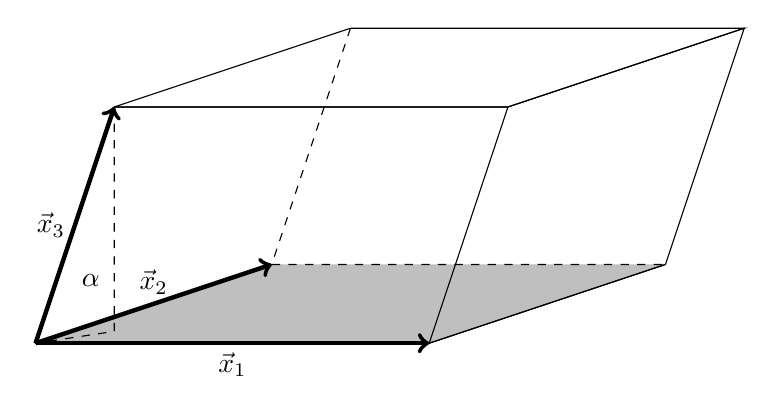
\begin{tikzpicture}
            \fill [lightgray] (0,0) -- (5,0) -- (8,1) -- (3,1);
            \draw [dashed] (4,4) -- (3,1) -- (8, 1);
            \draw (0,0) -- (5,0) -- (8,1);% -- (3,1);
            \draw (0,0) -- (5,0) -- (6,3) -- (1,3);
            \draw (1,3) -- (6,3) -- (9,4) -- (4,4);
            \draw (5,0) -- (8,1) -- (9,4) -- (6,3);
            \draw (3,1) -- (0,0) -- (1,3) -- (4,4);
            \draw [ultra thick, ->] (0,0) -- (5,0);
            \draw [ultra thick, ->] (0,0) -- (3,1);
            \draw [ultra thick, ->] (0,0) -- (1,3);
            \node [below] at (2.5, 0) {$\vec{x}_1$};
            \node [above] at (1.5, 0.5) {$\vec{x}_2$};
            \node [left] at (0.5, 1.5) {$\vec{x}_3$};
            \draw [dashed] (1,3) -- (1, 0.15) -- (0,0);
            \centerarc[] (0,0) (8:71.5:0.8);
            \centerarc[] (0,0) (8:71.5:0.87);
            \node at (0.7, 0.8) {$\alpha$};
        \end{tikzpicture}
    \end{center}
    За відомими формулами, об'єм $\Pi_m$ в цьому випадку дорівнює добутку площі основи на висоту паралелепіпеда.
    Основа --- це паралелепіпед $\Pi_{m \backslash j}$, а висота дорівнює $\Vert \vec{x}_3 \Vert \sin \alpha$.

    Повернемося до $\mathrm{tr} A^{-1} \leq \frac{m\cdot\Delta}{\det A} = 
    \frac{m\cdot\Delta}{\Delta \cdot \Vert \vec{x}_j \Vert^2 \sin^2 \alpha} = 
    \frac{m}{\Vert \vec{x}_j \Vert^2 \sin^2 \alpha}$.
    Без втрати загальності можна вважати, що $\exists \; \delta > 0$ таке, що 
    $\left|x_i^{(j)}\right| \geq \delta$ для всіх $i$ та $j$. Якби такого $\delta$
    не існувало, можна було б <<зсунути>> всі значення факторів так, щоб воно існувало.
    Це не надто вплине на модель, оскільки усі зсуви врахуються у вільному коефіцієнті.
    З цього випливає, що діагональні елементи $A$ необмежено зростають, а отже --- зростає їх сума, що дорівнює сумі власних чисел.
    Оскільки власні числа завжди додатні, то зростає і їх добуток, тому $\det A \to \infty$, $n\to\infty$.
    З цього, зокрема, випливає, що $\sin\alpha$ теж завжди залишається обмеженим знизу.
   
    Отже, $\frac{m}{\Vert \vec{x}_j \Vert^2 \sin^2 \alpha} \to 0, n\to\infty$, а тому й
    $\sum\limits_{k=1}^m \D\beta_k^* = \mathrm{tr}A^{-1} \to 0, n\to\infty$. Це, нарешті, доводить конзистентність оцінок $\beta_1^*, ..., \beta_m^*$.
\end{proof}

\subsection{Оцінка дисперсії похибок спостережень}
Нагадаємо, що дисперсії похибок спостережень $\sigma^2$ вважаються однаковими, але невідомими. В такому випадку для аналізу регресійної моделі
необхідно знайти оцінку $(\sigma^2)^*$. Зробимо це за допомогою методу максимальної правдоподібності: $\vec{\varepsilon} \sim \mathrm{N}(\vec{0}, \sigma^2 \mathbb{I}_n)$,
тому
\begin{gather*}
    \mathcal{L}(\vec{\eta}, \vec{\beta}, \sigma^2) = \frac{1}{(\sqrt{2\pi} \sigma)^n} \exp \left\{ 
        -\frac{1}{2\sigma^2} \sum\limits_{i=1}^n \left(\eta_i - f\left(\vec{x}^{(i)}\right)\right)^2
    \right\} \\
    \frac{\partial \ln \mathcal{L}}{\partial (\sigma^2)} (\vec{\eta}, \vec{\beta}, \sigma^2) 
    = -\frac{n}{2\sigma^2} + \frac{1}{2\sigma^4} \sum\limits_{i=1}^n \left(\eta_i - f\left(\vec{x}^{(i)}\right)\right)^2 = 0 \Rightarrow \\ \Rightarrow
    (\sigma^2)^* = \frac{1}{n} \sum\limits_{i=1}^n \left(\eta_i - f^*\left(\vec{x}^{(i)}\right)\right)^2 =
    \frac{1}{n} \Vert \vec{\eta} - F \vec{\beta}^* \Vert^2 = \frac{1}{n} \Vert \vec{\varepsilon}^{\,*}\Vert^2
\end{gather*}
\begin{definition}
    Вираз $\frac{1}{n} \Vert \vec{\varepsilon}^{\,*}\Vert^2$ називається \emph{залишковою оцінкою дисперсії} або
    \emph{залишковою сумою квадратів}.
\end{definition}
Перед знаходженням розподілу $(\sigma^2)^*$ розглянемо $m$-вимірний вектор $\sqrt{A}(\vec{\beta}^* - \vec{\beta})$ та його числові характеристики:
\begin{gather*}
    \E \left(\sqrt{A}(\vec{\beta}^* - \vec{\beta})\right) = \sqrt{A} \E \left(\vec{\beta}^* - \vec{\beta}\right) = \vec{0} \\
    \K \left(\sqrt{A}(\vec{\beta}^* - \vec{\beta})\right) = \sqrt{A} \cdot \K \left(\vec{\beta}^* - \vec{\beta}\right) \cdot (\sqrt{A})^T = 
    \sqrt{A} \cdot \sigma^2 A^{-1} \cdot \sqrt{A} = \sigma^2 \cdot \mathbb{I}_m
\end{gather*}
Отже, $\frac{1}{\sigma} \sqrt{A}(\vec{\beta}^* - \vec{\beta}) \sim \mathrm{N}(\vec{0}, \mathbb{I}_m)$. Повернемося до пошуку розподілу $(\sigma^2)^*$.
За побудовою вектор $\vec{\eta} - F \vec{\beta}^*$ є ортогональним до векторів виду $F\vec{x}$, $\vec{x} \in \mathbb{R}^m$, а тому й буде ортогональним до 
$F(\vec{\beta}^* - \vec{\beta})$. Тоді за теоремою Піфагора
\begin{gather*}
    \left\Vert \vec{\eta} - F \vec{\beta}^* \right\Vert^2 + \left\Vert F(\vec{\beta}^* - \vec{\beta}) \right\Vert^2 = 
    \left\Vert \vec{\eta} - F \vec{\beta}^* + F(\vec{\beta}^* - \vec{\beta})\right\Vert^2 = 
    \left\Vert \vec{\eta} - F \vec{\beta}\right\Vert^2 = \left\Vert \vec{\varepsilon}\right\Vert^2
\end{gather*}
Звідси $\Vert \vec{\eta} - F \vec{\beta}^* \Vert^2 = \Vert \vec{\varepsilon}\Vert^2 - \Vert F(\vec{\beta}^* - \vec{\beta}) \Vert^2$.
Розглянемо другий доданок цієї різниці:
\begin{gather*}
    \left\Vert F(\vec{\beta}^* - \vec{\beta}) \right\Vert^2  = \left(F(\vec{\beta}^* - \vec{\beta})\right)^T \left(F(\vec{\beta}^* - \vec{\beta})\right) = 
    (\vec{\beta}^* - \vec{\beta})^T F^T F (\vec{\beta}^* - \vec{\beta}) = \\ = 
    (\vec{\beta}^* - \vec{\beta})^T \sqrt{A} \cdot \sqrt{A} (\vec{\beta}^* - \vec{\beta}) = 
    \left(\sqrt{A}(\vec{\beta}^* - \vec{\beta})\right)^T \left(\sqrt{A}(\vec{\beta}^* - \vec{\beta})\right) =
    \left\Vert \sqrt{A}(\vec{\beta}^* - \vec{\beta}) \right\Vert^2 = \\ = 
    \left[\vec{\beta}^* - \vec{\beta} = A^{-1} F^T \vec{\varepsilon}\right] = 
    \left\Vert (\sqrt{A})^{-1} F^T \vec{\varepsilon} \right\Vert^2
\end{gather*}
Оскільки $\frac{1}{\sigma} \sqrt{A}(\vec{\beta}^* - \vec{\beta}) \sim \mathrm{N}(\vec{0}, \mathbb{I}_m)$, то й
$\frac{1}{\sigma}(\sqrt{A})^{-1} F^T \vec{\varepsilon} \sim \mathrm{N}(\vec{0}, \mathbb{I}_m)$, тому $\left\Vert \frac{1}{\sigma} (\sqrt{A})^{-1} F^T \vec{\varepsilon}\, \right\Vert^2 \sim \chi^2_m$.
Аналогічно, $\frac{1}{\sigma} \vec{\varepsilon} \sim \mathrm{N}(\vec{0}, \mathbb{I}_n)$ та 
$\left\Vert\frac{1}{\sigma} \vec{\varepsilon}\,\right\Vert^2 \sim \chi^2_n$.
Отже, $\frac{n (\sigma^2)^*}{\sigma^2} = \left\Vert\frac{1}{\sigma} \vec{\varepsilon}\,\right\Vert^2 - \left\Vert \frac{1}{\sigma} (\sqrt{A})^{-1} F^T \vec{\varepsilon}\, \right\Vert^2 \sim \chi^2_{n-m}$.
За властивостями розподілу хі-квадрат, $\E\left(\frac{n (\sigma^2)^*}{\sigma^2}\right) = n-m$, тому $\E(\sigma^2)^* = \frac{n-m}{n} \sigma^2$ і треба вводити виправлену незміщену оцінку 
$(\sigma^2)^{**} = \frac{n}{n-m}(\sigma^2)^*$. Таким чином, маємо незміщену оцінку дисперсії $\sigma^2$:
\begin{gather}
    (\sigma^2)^{**} = \frac{1}{n-m} \left\Vert \vec{\eta} - F \vec{\beta}^* \right\Vert^2
\end{gather}

Надалі для дослідження побудованої регресійної моделі знадобиться статистика
\begin{gather*}
    \vec{\gamma} = \frac{
        \frac{1}{\sigma} \sqrt{A}(\vec{\beta}^* - \vec{\beta})
    }{
        \sqrt{\frac{1}{n-m} \left(\frac{n (\sigma^2)^*}{\sigma^2}\right)}
    } = \frac{\sqrt{A}(\vec{\beta}^* - \vec{\beta})}{\sqrt{(\sigma^2)^{**}}}
\end{gather*}
Оскільки координати $\frac{1}{\sigma} \sqrt{A}(\vec{\beta}^* - \vec{\beta})$ є стандартними гауссівськими величинами,
то за аналогією з теоремою Фішера (ст. \pageref{Fisher_th}), $\gamma_i \sim \mathrm{St}_{n-m}, \; i = 1,..., m$.

\subsection{Перевірка адекватності моделі}
Після побудови регресійної моделі її перевіряють на \emph{адекватність}.
Це означає, що значення відклику, що прогнозуються моделлю, узгоджуються з результатами спостережень.

Одним із способів такої перевірки є так званий $\rm F$-критерій: порівняння \emph{залишкової оцінки дисперсії} $(\sigma^2)^{**}$, що обумовлена
випадковими помилками вимірів та, можливо, неврахованими факторами, з 
\emph{незміщеною оцінкою дисперсії} $\D^{**}\eta$. Оскільки
\begin{gather*}
    \frac{n-m}{\sigma^2} (\sigma^2)^{**}= 
    \frac{n}{\sigma^2}(\sigma^2)^* = \frac{1}{\sigma^2} \left\Vert \vec{\eta} - F \vec{\beta}^*\right\Vert^2 \sim \chi^2_{n-m} \\
    \frac{n-1}{\sigma^2} \D^{**}\eta = \frac{n}{\sigma^2} \D^* \eta = \frac{1}{\sigma^2} \sum\limits_{k=1}^n \left(\eta_k - \overline{\eta}\right)^2 \sim \chi^2_{n-1}
\end{gather*}
то розглядається статистика
\begin{gather}\label{f_test}
    \zeta = \frac{
        \frac{1}{n-1} \sum\limits_{k=1}^n \left(\eta_k - \overline{\eta}\right)^2
    }{
        \frac{1}{n-m} \left\Vert \vec{\eta} - F \vec{\beta}^*\right\Vert^2
    } = 
    \frac{
        \frac{1}{n-1} \sum\limits_{k=1}^n \left(\eta_k - \overline{\eta}\right)^2
    }{
        \frac{1}{n-m} \sum\limits_{k=1}^n \left(\eta_k - f^*\left(\vec{x}^{(k)}\right)\right)^2
    } \sim \mathrm{F}(n-1, n-m)
\end{gather}
У прикладі на ст. \pageref{intercept_fit} було показано, що якщо не включати
в регресійну модель жодних факторів, окрім константи, то оцінкою цього єдиного коефіцієнта буде $\overline{\eta}$.
Таким чином, $\rm F$-критерій перевіряє, чи є побудована регресійна модель кращою за найпростішу --- константну.
\emph{Основною гіпотезою} є те, що константа та побудована моделі не відрізняються (в тому сенсі, що дисперсії їх похибок однакові),
а \emph{альтернативною} --- що побудована модель є кращою за константну.
За заданим рівнем значущості треба знайти межу критичної області
$t_\text{кр}$. Критична область є правосторонньою: при $\zeta_\text{зн} > t_\text{кр}$ основна гіпотеза відхиляється і
модель вважається адекватною: це означає, що її дисперсія значно менше, ніж дисперсія моделі-константи.
Якщо основна гіпотеза не відхиляється, то треба спробувати додати в модель інші фактори.

Після перевірки на адекватність корегувати побудовану модель можна за допомогою перевірки \emph{гіпотези
про значущість параметрів}. Якщо значення якоїсь з оцінок $\beta_j^*$ виявилася близькою до нуля,
це може означати, що відповідний фактор не вносить внеску до моделі.
Висувається основна гіпотеза $H_0 : \beta_j = 0$ та альтернативна $H_1 : \beta_j < 0$ чи
$H_2 : \beta_j > 0$ в залежності від знаку отриманої оцінки $\beta_j^*$.
Оскільки $\vec{\beta}^* \sim \mathrm{N}(\vec{\beta}, \sigma^2 A^{-1})$,
то $\beta_j^* \sim \mathrm{N}(\beta_j, \sigma^2 a_{jj})$, де $a_{jj}$ --- елемент $A^{-1}$. Відповідно,
статистикою для перевірки гіпотези є 
\begin{gather}\label{signif_test}
    \gamma = 
    \frac{\beta_j^* }{\sqrt{(\sigma^2)^{**} \cdot a_{jj}}} \sim \mathrm{St}_{n-m}
\end{gather}
За заданим рівнем значущості треба знайти межу критичної області, яка буле правосторонньою чи лівосторонньою в залежності
від альтернативної гіпотези. Якщо основна гіпотеза $H_0 : \beta_j = 0$ приймається, то
відповідний фактор прибирається з моделі, але нову модель потрібно знову перевіряти на адекватність.

Таким чином, перевірка адекватності моделі за $\rm F$-критерієм показує,
чи не треба додати більше факторів, а перевірка значущості близьких до нуля параметрів ---
чи не треба зменшити кількість факторів.

\subsection{Аналіз точності прогнозів моделі}
Нехай побудована регресійна модель перевірена на адекватність та значущість параметрів.
Однією з задач, для яких її можна застосувати --- \emph{прогнозування значення відклику}
з тими значеннями факторів, з якими експеримент не проводився.
Аналіз точності отриманих прогнозів відбувається за допомогою побудови
довірчих інтервалів для самого значення відклику та його середнього значення.

Позначимо $f^*(\vec{x}) = \sum\limits_{i=0}^m \beta_i^* x_i$. 
$\E f^*(\vec{x}) = \sum\limits_{i=0}^m \E\beta_i^* x_i = \sum\limits_{i=0}^m \beta_i x_i = f(\vec{x})$
називається \emph{середнім значенням відклику}. Можна записати
$f^*(\vec{x}) = \vec{x}^{\, T} \vec{\beta}^*$ та $f(\vec{x}) = \vec{x}^{\, T} \vec{\beta}$, тоді
\begin{gather*}
    \D f^*(\vec{x}) = \E \left(\vec{x}^{\, T} (\vec{\beta}^* - \vec{\beta})\right)^2 = 
    \E \left(\vec{x}^{\, T} (\vec{\beta}^* - \vec{\beta})\right)\left(\vec{x}^{\, T} (\vec{\beta}^* - \vec{\beta})\right)^T = 
    \E\left(\vec{x}^{\, T} (\vec{\beta}^* - \vec{\beta}) (\vec{\beta}^* - \vec{\beta})^T \vec{x}\right) = \\
    = \vec{x}^{\, T} \E (\vec{\beta}^* - \vec{\beta}) (\vec{\beta}^* - \vec{\beta})^T \vec{x} = 
    \vec{x}^{\, T} \K\vec{\beta}^* \vec{x} = 
    \sigma^2 \vec{x}^{\, T} A^{-1} \vec{x}
\end{gather*}
Отже, маємо статистику
$
    \frac{f^*(\vec{x}) - f(\vec{x})}{\sigma \sqrt{\vec{x}^{\, T} A^{-1} \vec{x}}} \sim \mathrm{N}(0, 1)
$. Оскільки $\frac{n-m}{\sigma^2} (\sigma^2)^{**} \sim \chi^2_{n-m}$, то
\begin{gather*}
    \zeta = \frac{
        \frac{f^*(\vec{x}) - f(\vec{x})}{\sigma \sqrt{\vec{x}^{\, T} A^{-1} \vec{x}}}
    }{
        \sqrt{
            \frac{1}{n-m}\cdot \frac{n-m}{\sigma^2} (\sigma^2)^{**}
        }
    } = \frac{f^*(\vec{x}) - f(\vec{x})}{
        \sqrt{(\sigma^2)^{**} \vec{x}^{\, T} A^{-1} \vec{x}}
    } \sim \mathrm{St}_{n-m}
\end{gather*}
Для побудови довірчого інтервалу з рівнем надійності $\gamma$ за таблицею знаходять таке $t$, що
$\P\left\{|\zeta| < t \right\} = \gamma$. Довірчий інтервал для середнього значення відклику має вигляд
\begin{gather}\label{interv_1}
    f(\vec{x}) \in 
    \left(
        f^*(\vec{x}) - t \sqrt{(\sigma^2)^{**} \vec{x}^{\, T} A^{-1} \vec{x}}, 
        f^*(\vec{x}) + t \sqrt{(\sigma^2)^{**} \vec{x}^{\, T} A^{-1} \vec{x}}
    \right)
\end{gather}

Для побудови довірчого інтервалу для самого значення відклику скористаємося тим, що
$\E \left(\eta - f^*(\vec{x})\right) = 0$, а $\D\left(\eta - f^*(\vec{x})\right) = 
\D\eta + \D f^*(\vec{x}) = \sigma^2 \left(1 + \vec{x}^{\, T} A^{-1} \vec{x}\right)$. Аналогічними міркуваннями отримаємо
\begin{gather*}
    \frac{\eta - f^*(\vec{x})}{
        \sqrt{(\sigma^2)^{**} \left(1 + \vec{x}^{\, T} A^{-1} \vec{x}\right)}} \sim \mathrm{St}_{n-m}
\end{gather*}
тому довірчий інтервал для значення відклику матиме вигляд
\begin{gather}\label{interv_2}
    \eta \in
    \left(
        f^*(\vec{x}) - t \sqrt{(\sigma^2)^{**} \left(1 + \vec{x}^{\, T} A^{-1} \vec{x}\right)}, 
        f^*(\vec{x}) + t \sqrt{(\sigma^2)^{**} \left(1 + \vec{x}^{\, T} A^{-1} \vec{x}\right)}
    \right)
\end{gather}

\subsection{Приклад побудови та аналізу моделі}
За заданими значенням $y_i$ та $x_i$ знайти оцінки параметрів простої однофакторної лінійної регресійної
моделі $y = f(x) = \beta_0 + \beta_1 x$. Перевірити побудовану модель на адекватність та на значущість параметрів на рівні значущості $\alpha=0.05$.
Побудувати довірчі інтервали для середнього значення відклику та значення відклику в точці $x_0 = 10$ з рівнем надійності $0.99$.
\begin{center}
    \begin{tabular}{|c|c|c|c|c|c|c|c|c|c|c|}
        \hline
        $x_i$ & $2.7$ & $4.6$ & $6.3$ & $7.8$ & $9.2$ & $10.6$ & $12.0$ & $13.4$ & $14.7$ \\
        \hline
        $y_i$ & $17.0$ & $16.2$ & $13.3$ & $13.0$ & $9.7$ & $9.9$ & $6.2$ & $5.8$ & $5.7$ \\
        \hline
    \end{tabular}
\end{center}
\begin{center}
    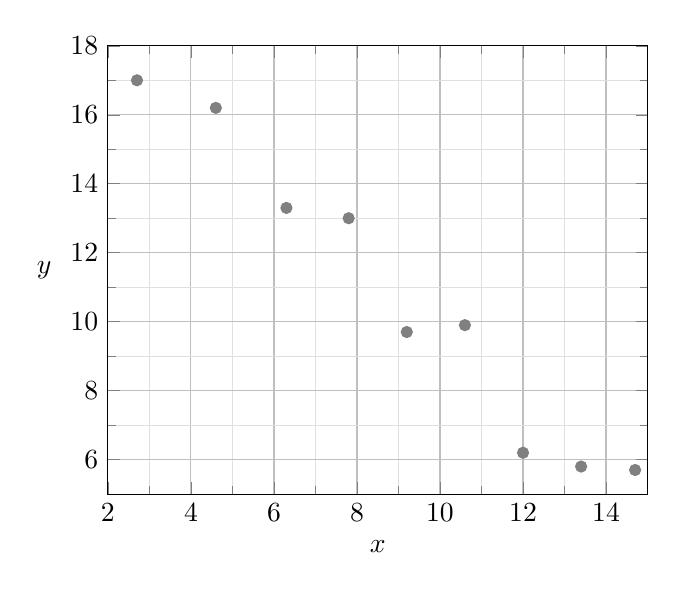
\begin{tikzpicture}
        \begin{axis}[
            xmin = 2, xmax = 15,
            ymin = 5, ymax = 18,
            xtick distance = 2,
            ytick distance = 2,
            grid = both,
            minor tick num = 1,
            major grid style = {lightgray},
            minor grid style = {lightgray!50},
            xlabel = {$x$},
            ylabel = {$y$},
            ylabel style={rotate=-90}]
            \addplot[gray, only marks] table {
                2.7     17.0
                4.6     16.2
                6.3     13.3
                7.8     13.0
                9.2     9.7
                10.6    9.9
                12.0    6.2
                13.4    5.8
                14.7    5.7
            };
        \end{axis}
    \end{tikzpicture}
\end{center}
Складемо матрицю плану $F = \begin{pmatrix}
    1 & 1 & \cdots & 1 \\
    2.7 & 4.6 & \cdots & 14.7
\end{pmatrix}^T$. Інформаційна та дисперсійна матриці дорівнюють, відповідно,
$A = F^T F= \begin{pmatrix}
    9 & 81.3 \\
    81.3 & 865.63
\end{pmatrix}$,
$A^{-1} = \begin{pmatrix}
    0.73298 & -0.06884 \\
    -0.06884 & 0.00762
\end{pmatrix}$. Вектор значень відкликів
$\vec{\eta}_\text{зн} = \begin{pmatrix}
    17.0 & 16.2 & \cdots & 5.7
\end{pmatrix}^T$, тому можемо знайти значення оцінок параметрів моделі:
\begin{gather*}
    \vec{\beta}^*_\text{зн} = A^{-1} F^T \vec{\eta}_\text{зн} \approx \begin{pmatrix}
        20.30566 \\ -1.05721
    \end{pmatrix}
\end{gather*}
Отже, маємо модель $y = f^*(x) = 20.30566 -1.05721 x$, графік якої зображено нижче.
\begin{center}
    \begin{tikzpicture}
        \begin{axis}[
            xmin = 2, xmax = 15,
            ymin = 5, ymax = 18,
            xtick distance = 2,
            ytick distance = 2,
            grid = both,
            minor tick num = 1,
            major grid style = {lightgray},
            minor grid style = {lightgray!50},
            xlabel = {$x$},
            ylabel = {$y$},
            ylabel style={rotate=-90}]
            \addplot[gray, only marks] table {
                2.7     17.0
                4.6     16.2
                6.3     13.3
                7.8     13.0
                9.2     9.7
                10.6    9.9
                12.0    6.2
                13.4    5.8
                14.7    5.7
            };
            \addplot[ultra thick] table[
                x = t,
                y = {create col/linear regression={y=x}}
            ] {
                t       x
                2.7     17.0
                4.6     16.2
                6.3     13.3
                7.8     13.0
                9.2     9.7
                10.6    9.9
                12.0    6.2
                13.4    5.8
                14.7    5.7
            };
        \end{axis}
    \end{tikzpicture}
\end{center}

Перевіримо побудовану модель на адекватність. Обчислимо значення виправленої 
вибіркової дисперсії для $\eta$ та залишкову оцінку дисперсії:
$\left(\D^{**}\eta\right)_\text{зн} = \frac{1}{8}
\sum\limits_{i=1}^9 \left(y_i - \overline{y}\right)^2 \approx 19.1$, 
$(\sigma^2)^{**}_\text{зн} = \frac{1}{7}
\sum\limits_{i=1}^9 \left(y_i - f^*(x_i)\right)^2\approx 0.88564$.
Значення статистики $\rm F$-критерію (\ref{f_test}) $\zeta_\text{зн} \approx 21.5752$.
За таблицею знайдемо межу критичної області для $\mathrm{F}(8, 7)$: $t_\text{кр} = 3.73$.
Отже, $\zeta_\text{зн} > t_\text{кр}$ і модель можна вважати адекватною на рівні значущості $0.05$.

Перевіримо значущість параметра $\beta_2$. Основною гіпотезою є $H_0 : \beta_2 = 0$,
альтернативною --- $H_1 : \beta_2 < 0$. Знайдемо значення відповідної статистики
(\ref{signif_test}): $\gamma_\text{зн} = \frac{
    -1.05721
}{
    \sqrt{0.88564 \cdot 0.00762}
} \approx - 12.87$. 
За таблицею знайдемо межу критичної області для $\mathrm{St}_7$: $t_\text{кр} = -1.895$.
Отже, $\gamma_\text{зн} < t_\text{кр}$ і основна гіпотеза відхиляється, тому параметр $\beta_2$ є значущим.

Для знаходження обох довірчих інтервалів знайдемо 
$\vec{x}^{\, T} A^{-1} \vec{x}$ для $\vec{x} = \begin{pmatrix}
    1 \\ 10
\end{pmatrix}$ та $f^*(x_0)$. Отримані значення --- $0.11823$ та $9.7336$ відповідно.
За таблицею знайдемо для $\mathrm{St}_7$ значення $t = 3.499$, тому за формулою
(\ref{interv_1}) отримаємо довірчий інтервал для середнього значення відклику в точці $x_0 = 10$:
\begin{gather*}
    f^*(x_0) \pm t \sqrt{(\sigma^2)^{**}_{\text{зн}} \vec{x}^{\, T} A^{-1} \vec{x}} =
    9.7336 \pm 3.499\cdot\sqrt{0.88564 \cdot 0.11823} \approx 9.7336 \pm 1.13223 \\
    f(\vec{x}) \in 
    \left(
        8.60137, 
        10.86583
    \right) \approx \left(8.6, 10.87\right)
\end{gather*}
За формулою (\ref{interv_2}) отримаємо довірчий інтервал для значення відклику в точці $x_0 = 10$:
\begin{gather*}
    f^*(x_0) \pm t \sqrt{(\sigma^2)^{**}_{\text{зн}}\left(1 + \vec{x}^{\, T} A^{-1} \vec{x}\right)} = 
    9.7336 \pm 3.499\cdot\sqrt{0.88564 \cdot 1.11823} \approx 9.7336 \pm 3.482 \\
    \eta_\text{зн} \in \left(6.2516, 13.2156\right) \approx \left(6.25, 13.22\right)
\end{gather*}
Такі широкі довірчі інтервали пояснюються, зокрема, малим обсягом вибірки.

\subsection{Деякі труднощі застосування лінійної регресійної моделі}
Одне з основних припущень для застосування лінійної регресійної моделі $\vec{\varepsilon} \sim \mathrm{N}(\vec{x}, \sigma^2 \mathbb{I})$ є доволі
<<жорстким>> і не завжди виправданим: наприклад, дисперсії похибок можуть змінюватися в залежності від значень факторів.

Також, складним іноді може бути вибір кількості факторів. З одного боку, включення до моделі
багатьох факторів може як підвищити її точність, так і погіршити оцінки параметрів, оскільки деякі фактори
можуть бути лінійно залежними (або близькими до таких), що призведе до виродженості чи поганої обумовленості матриці $A$ --- таке 
явище називається \emph{мультиколінеарністю} факторів. На практиці ще перед побудовою моделі часто
досліджують зміст самих факторів (наприклад, щоб не включати два фактори, один з яких показуватиме 
вимірювання деякої величини в метрах, а інший --- в сантиметрах), а також вибіркові коефіцієнти кореляції між факторами:
якщо значення цього коефіцієнту для якихось двох факторів буде близьким за модулем до 1,
то, скоріш за все, вони є лінійно залежними, тому один із них не варто включати до моделі.

Іншим припущенням при побудові лінійної регресійної моделі є лінійна за параметрами
залежність середнього значення відклику від значень факторів. Якщо все ж таки нелінійність очевидна (наприклад, з погляду на \emph{діаграму розсіювання}),
то треба застосовувати якесь перетворення змінних. Наприклад, розглянемо дві діаграми розсіювання:
\begin{center}
    \begin{tabular}{c c}
        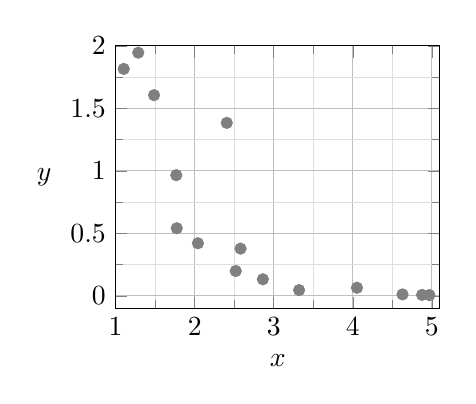
\begin{tikzpicture}
            \begin{axis}[
                xmin = 1, xmax = 5.1,
                ymin = -0.1, ymax = 2,
                xtick distance = 1,
                ytick distance = 0.5,
                width = \textwidth*0.47,
                grid = both,
                minor tick num = 1,
                major grid style = {lightgray},
                minor grid style = {lightgray!50},
                xlabel = {$x$},
                ylabel = {$y$},
                ylabel style={rotate=-90}]
                \addplot[gray, only marks] table {
                    1.77351 0.54076
                    3.32050 0.04585
                    1.48636 1.60510
                    2.51957 0.19826
                    1.10318 1.81498
                    2.86248 0.13232
                    4.62895 0.01131
                    2.40601 1.38353
                    4.87574 0.00739
                    4.96824 0.00579
                    2.58016 0.37752
                    1.76736 0.96512
                    1.28632 1.94514
                    4.05253 0.06455
                    2.04099 0.42063
                };
            \end{axis}
        \end{tikzpicture} &
        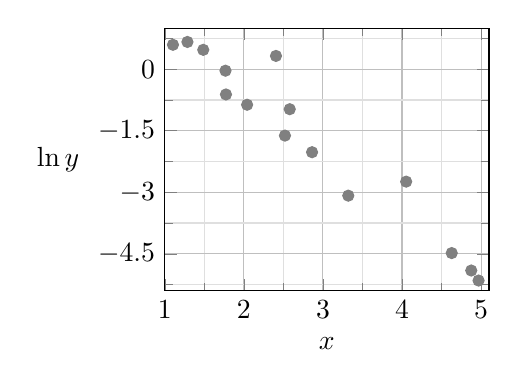
\begin{tikzpicture}
            \begin{axis}[
                xmin = 1, xmax = 5.1,
                ymin = -5.4, ymax = 1,
                xtick distance = 1,
                ytick distance = 1.5,
                width = \textwidth*0.47,
                grid = both,
                minor tick num = 1,
                major grid style = {lightgray},
                minor grid style = {lightgray!50},
                xlabel = {$x$},
                ylabel = {$\ln y$},
                ylabel style={rotate=-90}]
                \addplot[gray, only marks] table {
                    1.77351 -0.61479
                    3.32050 -3.08228
                    1.48636 0.47318
                    2.51957 -1.61818
                    1.10318 0.59608
                    2.86248 -2.02256
                    4.62895 -4.48196
                    2.40601 0.32464
                    4.87574 -4.90751
                    4.96824 -5.15177
                    2.58016 -0.97412
                    1.76736 -0.03550
                    1.28632 0.66533
                    4.05253 -2.74033
                    2.04099 -0.86600
                };
            \end{axis}
        \end{tikzpicture}
    \end{tabular}
\end{center}
Видно, що логарифмування змінної $y$ дало залежність, що схожа на лінійну. В такому випадку
будується модель виду $z = \ln y = \beta_0 + \beta_1 x$, звідки потім отримується $y = e^{\beta_0 + \beta_1 x}$.

Насамкінець, важливо зауважити, що методи регресійного аналізу
дозволяють з'ясувати \emph{лише числові залежності} --- як значення деяких величин 
впливає на середнє значення іншої. Причинно-наслідкові зв'язки цими методами дослідити неможливо.
Наприклад, між віком будинку та ціною квартир в ньому можна знайти деякий кореляційний зв'язок. 
Чи можна з цього зробити висновок, що чим дорожча квартира, тим новіше будинок, в якому вона знаходиться? Ні.
Але можна перевірити, як вік будинку впливає на середню ціну квартир --- на це питання регресійний аналіз вже може дати відповідь. 